\documentclass[   
state        = Thesis,                       % (Report | Thesis)
lang         = EN,                           % (DE     | EN) 
degree       = MSc,                          % (BSc    | MSc)
dept         = MECH,                         % (MECH   | SBT)
bib-active   = true,                         % (true   | false)
bib-style    = ieee,                         % (ieee)
column-type  = two,                          % (one    | two)
]{mcidoc}

% CUSTOM COMMANDS -----------------------------------------------------------------------------
%       
% Please enter any custom command/packages you require here for easy tracking 
  
% For example, bibliography setting are added. Bibtex is the standard but if you prefer
% there are other options on the market such as biber. Style has been chosen as IEEE but if 
% are from another discipline, please feel free to change it.


 
 
\bibliography{references.bib}  % Here we add our file where we store our references.
%      
% ---------------------------------------------------------------------------------------------

% DOCUMENT PARAMETERS -------------------------------------------------------------------------

\Title{%
  On the Study of Different Rotor Geometry Configuration for use in High-Speed
  Induction Motors
}% 
 
\StudentName{Jason Smith} 
\StudentID{2024000095} 
            
\StudyProgram{Mechatronics \& Smart Technologies}  
\Supervisor{Colin Stevens}

\begin{document} % ############################################################################
                 
\MakeTitlePage     
 
\DeclarationOfNovelty

\ThesisEmbargoRequest[5]
 
\TableOfContents  
 
% REPORT CONTENT ------------------------------------------------------------------------------
               
% ----      
% Your report content should go here and should follow structure befitting of a scientific
% report and should be written in a scientific format. For more information please look at
% MCI guidelines on how it should be done.      
% ----  
             
% Include Chapter - introduction
\chapter{Introduction}

\section{The Need for Speed}

In recent years, improvements in manufacturing, transportation and process industry
technologies bring about an increase in optimal operation speed in drive systems. In this
respect, recently developed high speed gear-less or direct-drive electrical drives have seen an
increase in interest based on the reduction in the total structural volume of the drive
system. Due to the significant development of cost-effective, fast switching and compact
variable frequency drives technology, wide speed range operations of different type AC motors
has become feasible. The speed definition of an induction motor can be seen in Eq.\ \ref{eq:speed}

\begin{equation}  \label{eq:speed}
  n = \frac{120 f}{p},
\end{equation}

In literature, there are several descriptions for the term "high-speed".  As a mechanical
engineer, peripheral speed over \SI{150}{\meter\per\second} is considered to be high speed
\cite{gieras2011performance}. From the motor manufacturer's point of view, a two-pole machine
which is supplied higher than 50 to \SI{60}{\hertz}, can be considered as a high-speed machine.
However, the most important point of view for the high-speed term is explained by development
at power electronics. Nowadays, up to few hundreds hertz frequencies can be produced by
variable frequency drives. However, voltage qualities of these are not satisfactory due to
limited switching frequency of high-power IGBT technology. Thus, high-speed levels might be
calculated for frequencies in the range of 100 to \SI{400}{\hertz} are considered to be
high-frequencies \cite{pyrhonen1991high}.  Owing to brush and commutator structure causing mechanical and
electrical problems, DC drives are not allowed to be used for high-speed applications. In
addition to the aforementioned statement, the structure is not appropriate for large
centrifugal forces.  Nevertheless, as high-speed drive applications, there are different type
of AC motor concepts proposed in literature
\cite{gieras2011performance, pyrhonen1991high, lahteenmaki2002design, saari1998thermal}:
Laminated/solid induction, permanent
magnet synchronous and switched reluctance synchronous motors.

\begin{table}
  \begin{tabular}{rll} \toprule
    \parbox[t]{5cm}{\textbf{Admission requirements                            \\ for Mathematics (MSc)}}  & \parbox[t]{5cm}{\textbf{Courses completed \\ before start}} & \parbox[t]{2.5cm}{\textbf{Date of \\ completion}} \\  \midrule
    Mathematical Analysis (30 ECTS)    & Mathematical Analysis 1 & 22.04.2014 \\
    ~                                  & Mathematical Analysis 2 & 15.02.2013 \\
    ~                                  & Complex Analysis        & 01.07.2015 \\ \midrule
    Algebra/Linear algebra (22.5 ECTS) & Advanced Algebra        & 17.02.2013 \\
    ~                                  & Abstract Algebra        & 01.06.2015 \\ \midrule
    Geometry/Topology (15 ECTS)        & Topology                & 01.11.2014 \\
    ~                                  & Vector Analysis         & 15.06.2015 \\
    ~                                  & Differential Geometry   & 15.02.2013 \\ \bottomrule
  \end{tabular}
  \caption{As can be clearly seen, this table has absolutely no reason to be here aside from
    taking space. But it is a nice table to show how it should look and a template to write your
    own tables.}
\end{table}

It is due to remarkable improvements of power electronics, frequency inverters and AC
variable-speed drives, which allows a wider use of applications of solid-rotor induction motor
(SRIM). SRIM's are used in drive application ranging from a few kW's to 10 MW's. Fans,
compressors, pumps, gas turbines, sewing machines, space and aeronautics, auxiliary motors for
starting turbo-alternators, eddy current brakes, two-phase servomotors are a few examples of its
areas. \\

Below are the advantages of SRIM compared to CRIM:

\begin{itemize}[itemsep=0pt]
\item Structural and Mechanical integrity, Rigiditiy, Reliability and Strength of
  Material
\item High thermal properties
\item High speed in high power applications (high moment density)
\item Low noise and vibrations in high speed applications
\item Simple to protect against aggressive chemicals
\item Ease of Manufacturing
\item Low level of noise and vibrations (If the rotor has no slots)
\item Linearity of torque-speed characteristics throughout the entire speed range
\item The possibility of obtaining steady-state stability.
\end{itemize}

In 1950s, Solid-Rotor topologies for induction machines operating at high speeds
have gained a lot of interest. From its inception to 1970s, various scientists and engineers
have contributed to the development and the theory of solid rotor construction, where significant
interest was seen the 1990s for using solid rotor structure for high speed applications.

\begin{figure}[!t]
  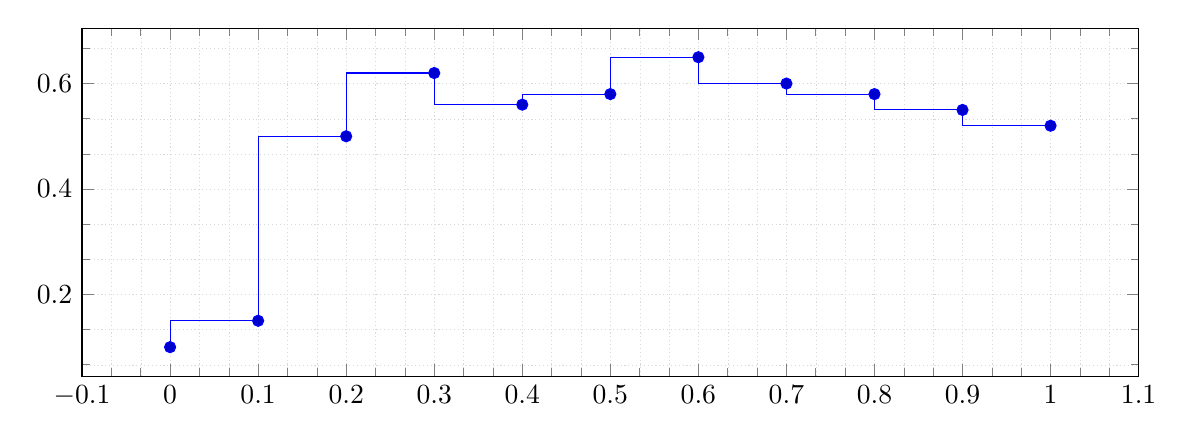
\begin{tikzpicture}
    \begin{axis}[width=15cm, height=6cm,
      minor tick num   = 2,
      grid             = both,	% have a grid that is bitchin
      % GRID OPTIONS
      minor grid style = {
        densely dotted,
        line width = 0.1,
        gray!30
      },
      major grid style={
        densely dotted,
        line width = 0.3,
        gray!30
      }]
      \addplot+ [
      const plot mark right,
      ] coordinates {
        (0,0.1)    (0.1,0.15)  (0.2,0.5)   (0.3,0.62)
        (0.4,0.56) (0.5,0.58)  (0.6,0.65)  (0.7,0.6)
        (0.8,0.58) (0.9,0.55)  (1,0.52)
      };
    \end{axis}
  \end{tikzpicture}
  \caption{The authors interest in the topic as years go on.}
\end{figure}

As the rotor does not contain any trace of copper \footnote{the rotor
  consists of a solid body of steel or similar ferromagnetic material}{windings}, the eddy currents
roam in the rotor without any conductive path restriction and cause the motor to
have different characteristics compared to a Cage Rotor Induction motor (CRIM), an industry standard
construction.
While eddy currents are the main principle of its operation, these currents also causes
the motor to have lower efficiency in slow speed aplications and this indirectly
decreases its power factor. But in high speed application where the speed is
around 30000 rpm the losses become far less and SRIM becomes the better choice for high speed
applications.

\subsection{Report Structure} %~~~~~~~~~~~~~~~~~~~~~~~~~~~~~~~~~~~~~~~~~~~~~~~~~~~~~~~~~~~~~~~~

In this report for Drive Technologies, the high-speed performance of the four
different types of rotors are investigated and compared using finite element analysis:
cage, smooth solid, axially slitted, coated is designed using a finite-element
analysis (FEA). All rotors are designed with similar geometries and construction parameters
to minimise the effect of unwanted effects.

\begin{lstlisting}[language=C++]  
  // C++ program to find all string
  // which are greater than given length k 

  #include <bits/stdc++.h> 
  using namespace std;

  // function find string greater than
  // length k 
  void string_k(string s, int k) 
  {
    // create an empty string
    string w = "";
    // iterate the loop till every space
    for (int i = 0; i < s.size(); i++) {
      if (s[i] != ' ')

      // append this sub string in
      // string w
      w = w + s[i];
      else {

        // if length of current sub
        // string w is greater than 
        // k then print
        if (w.size() > k)
        cout << w << " "; 
        w = "";
      }
    }
  }
\end{lstlisting}

The number of turns per stator slot is selected so as to obtain the
same stator current in rated operation. All four motors were analyzed using FEA
tools for 20 different speeds in order to obtain the combined torque-speed
characteristics. To illustrate visually the differences in the distributions of the
magnetic flux and the eddy current the results for 11300 rpm are presented and the
core loss, the total loss and the efficiency for the specific speed are compared for all
the motors. The designed four motors will be also compared for winding currents,
induced voltages, flux linkages, electromagnetic torque, copper losses, iron losses,
solid rotor losses and efficiency.
   
     
% Include Chapter - literature survey  (contains minted code)
%%

\chapter{Literature Review} %------------------------------------------------------------------
 

The term "high-speed" generally is used to define a motor that goes faster than 150 m/s
[2]. The mentioned speed can be achieved with a simple 2p = 2, 50 Hz machine with
around 1m diameter. Since the European grid is fed with 50 Hz AC it can achieve
only 3000 min-1. American grid can achieve 3600 min-1 since it uses 60 Hz AC. The
term has not have a solid cut-off point since some manufacturers put the limit on
3600 min-\footnote[2]{tt}
.       
1
The research in the field of high-speed machines has been mostly active in
Finland.[3] worked on ferromagnetic core matericals in smooth solid-rotors.[4]'s
topic was rotor designs and voltage sources suitable for high-speed machines. His
main research focus was the design of squirrel cage and coated solid rotors. [5]
studied high-speed induction machines thermal analysis and [6] was focused on air–
gap friction in high-speed machines.[7] and [8] worked on active magnetic bearings
used in high-speed induction machines. It must me noted that the research mentioned
above used machines that run on 100 Hz to 300 Hz.
Other dissertations have also been done on the field of solid rotor 
technology.[9] has studied on experimentally slitted solid rotors with 19 kW, 50 Hz,
2p = 4 induction motor. [10 11 12] has investigated the effects of axial slits, end
rings and cage windings in a solid ferromagnetic rotor with the values of 3 Hp
(around 2.23kW), 50 Hz, 2p = 6. Balarama Murt [13] has also made investigations
on axial slits on solid steel rotors. Woolley [14] studied new designs of unlaminated
rotors. Zaim [15] studied rotor concepts for induction motors.

In recent years the laboratory of electrical engineering at Lappeenranta University of
Technology (LUT) has done research on improving the efficiency of high-speed
solid-rotor construction. From this research it was found that when a solid-rotor is
used, the flux density distribution of the rotor surface plays a significant role. To
have the least amount of lossess, the rotor must have a perfectly sinusoidal rotor
surface. This also applies to time dependent and spatial harmonics. Research has
given promising results and the efficiency of these types of machines have increased
to the level comperable to a regular 3000 induction motor of same power
output.



  

The research at LUT got off with the study of a 12 kW, 400 Hz induction
motor [15]. Continuing from the research different types of rotor with different rotor
coatings and end rings with new stator design were used to improve the efficiency
[16]. From the successful results, 16 kW, 225 Hz induction motor with a smooth, a
slitted and a squirrel-cage solid rotors were experimented [17].
After these successful tests the focus was shifted to bigger machines. A 200
kW,140 Hz slitted Solid-Rotor induction machine and a 250 kW, 140 Hz slitted solid
rotor with copper end rings were analyzed [18].
It is known that by axially slitting the motor, its electromagnetic properties
can be improved. This type of construction must be done in an optimal way. The
penetratino of the flux lines must be calculated and this is directly connected to the
slit width and depth. According to [19]'s reseach, the optimal values for the rotor is
half of the radius for the depth and 1,5 mm width.
The output torque of an electric machine is related and proportional to the
product of the Amperé-turns and the magnetic flux per pole. Because for a given
motor size the Amperé-turns and the magnetic flux per pole are limited, the most
efficient way to increase the output is to increase the speed.
According to [20] there is a correlation between eddy current lossess and the
coating material for CCIM. This research show that by using a material the is at least
twice as conductive as the coated material the eddy lossess are dramatically reduced.
The thickness for the coating is also an improtant design factor. As it is used to
concentrate eddy currents to the surface a proximal value must be chosen.[21] shows
that by picking a thickness of 1,5 mm copper material an optimal performance can be
gained.


The most attractive advantage of high-speed range is the reduction or the
motor size. The volume per power ratio and the weight per power ratio are inversely
proportional to the rotating speed in high-speed.
Solid-rotors are also used for their mechanical properties. This type of rotor
are the strongest type one can construct. It can also be used in very high-speeds since
it can maintain its balance well. When a load is directly attached to the shaft, the
solid rotor can still show an impressive mechanical durability and can avoid
vibrations.High-speed solid rotor induction motors may be used in applications from
a few kilowatts up to tens of megawatts. Their main area are where the laminated
rotor construction are not durable enough. [2] has defined the speed limits for certain
rotor.

The mechanical limit of laminated rotor rotational speed varies from 10.000
min-1 50.000 min-1 (to reach these speeds special constructions may be
demanded)
 The mechanical limit of solid-rotor rotational speed varies from 20.000 min-1
to 100.000 min-1 (to reach these speeds special constructions may be
demanded)

\begin{minted}{cpp}   
  // C++ program to find all string
  // which are greater than given length k 
  
  #include <bits/stdc++.h> 
  using namespace std;
  
  // function find string greater than
  // length k
  void string_k(string s, int k) 
  {
    // create an empty string
    string w = "";
    // iterate the loop till every space
    for (int i = 0; i < s.size(); i++) {
      if (s[i] != ' ')
      
      // append this sub string in
      // string w
      w = w + s[i];
      else {
        
        // if length of current sub
        // string w is greater than
        // k then print
        if (w.size() > k)
        cout << w << " ";
        w = "";
      }
    }
  }
\end{minted}



%%% Local Variables:
%%% mode: LaTeX
%%% TeX-master: "../Vorlage_thesis"
%%% End:
      
                  
% ---- 
% Add as many chapters as you see fit for your content. For easy legibility and for dynamic
% adjustment of content it would be suggested to write your files and place them similar to
% the aforementioned examples.

% REPORT POSTAMBLE ----------------------------------------------------------------------------

% ----
% In this section, please put all the thing you deem are necessary for the thesis but does have
% no substance as materials (i.e., technical drawings, patents, massive code bases).
% ----

\printbibliography

% \makeindex
% \printnomenclature
% \printglossaries

\end{document} % ##############################################################################
